\documentclass[twoside]{article}
\usepackage{mathpazo}
\usepackage[T1]{fontenc}
\usepackage[utf8]{inputenc}
\usepackage{graphicx}
\usepackage[colorlinks]{hyperref}
\hypersetup{
  colorlinks,
  urlcolor=blue,
  linkcolor=black
}
\usepackage{caption} % unnumbered video examples
% \usepackage{authblk} % author affiliations
\usepackage{hanging} % hanging indents

% headers
\usepackage{fancyhdr}
\renewcommand{\headrulewidth}{0pt}

% first page footer
\fancypagestyle{infofooter}{%
  \fancyhf{}
  \renewcommand\headrulewidth{0pt}
  \fancyfoot[L]{\sffamily\small 
    WORLD MUSIC TEXTBOOK, ISSN: 2767-4215; \copyright~2021, CC-ND-BY-ND\\
    http://dx.doi.org/XX.XXXX/XXXXXXXX.2021.XXXXXXX}
}
\thispagestyle{infofooter} % remove header from first page
\pagestyle{fancy}     % add headers in other pages

% normal headers
\fancyhead[LO]{\sffamily\small \textbf{\thepage} \quad World Music Textbook}
\fancyhead[RE]{\sffamily\small Witulski: Rhythm and expectation \quad \textbf{\thepage}}
\fancyfoot{}

% flush left title
\makeatletter
\renewcommand{\maketitle}{\bgroup\setlength{\parindent}{0pt}
\begin{flushleft}
  \vspace*{3\baselineskip}
  \huge{\textbf{\@title}}

  \medskip
  
  \large{\@author}
\end{flushleft}\egroup
}
\makeatother

% for keywords and abstract
\providecommand{\abstracttext}[1]
{
  \noindent
  \textbf{Abstract:} #1
}

\providecommand{\keywords}[1]
{
  \newline
  \textbf{Keywords:} #1
}

% for link
\providecommand{\wmturl}{\href{https://worldmusictextbook.org/witulski-rhythm}{https://worldmusictextbook.org/witulski-rhythm}}
\providecommand{\wmturltext}{
  \noindent\emph{The online version of this chapter includes all embedded content and is available at \wmturl.}
}
\providecommand{\wmturlcaption}{
  Scan the QR code or visit \href{https://worldmusictextbook.org/witulski-rhythm}{the website} to view.
}

% metadata
\title{Rhythm and Expectation}
\author{Christopher Witulski | Bowling Green State University}
% \affil{}

\date{}

\begin{document}

\suppressfloats % prevent float above title
\maketitle

\abstracttext{This four-part series\footnote{This originated online and is split into multiple separate parts. They are combined into a single PDF here for convenience. Some links may break over time, but the online versions will remain updated.} explores the relationship between rhythm, expectation, and experience. It describes musical terms and central concepts while using specific examples from Morocco to problematize western-centric binaries.}
\keywords{musical terms, sound, Africa, global, Middle East}

\smallskip

\wmturltext

\medskip

\noindent\hfil\rule{0.5\textwidth}{0.4pt}\hfil

\bigskip

This set of short essays describes core elements of rhythm by
prioritizing perception with three goals in mind. First, I aim to
introduce some terminology that can inform how we hear and understand
what we listen to. These elements may prove more or less helpful
depending on the music that is playing, but they are widely applicable.

Second, the approaches here resist the western-centric methods and
perspectives that commonly define things like beat, meter, and
subdivision. The examples that I present---especially the ones in the
final section, where I draw from my own research in Morocco---show how
western perspectives are not as widely useful as they are often assumed
to be. Like other global musical systems, western musical notation is
derived from specific histories and compositional styles. It is a tool
serving a purpose, one that is usually related to the preservation of
specific elements of a composition for the sake of performance. Even
within the context of western classical music, it hinders certain
nuances of performance practice when used inappropriately. For this
reason, I define concepts broadly with the hope that they may prove more
useful across a range of musics and experiences.

And, speaking of experience, I want to focus our understanding of music
and sound more holistically on the body. We do not just hear music, we
feel it, dance it, sing it, and hear to the world around us through it.
Yet, each of us does so differently based on our own experiences,
abilities, training, hopes, dreams, and so on.

These essays are organized into four parts. The first introduces some
basic concepts of rhythm through the lens of expectation. The second
addresses repetition and meter using cycles, again drawing on
expectation. The third moves to the micro-level by discussing beat and
timing and how they impact the way we feel music. The final part uses
these ideas of rhythm, expectation, and repetition to introduce and
analyze three rhythmic patterns from Moroccan sacred musics that resist
easy definition according to western perspectives.

\begin{figure}
  \centering
  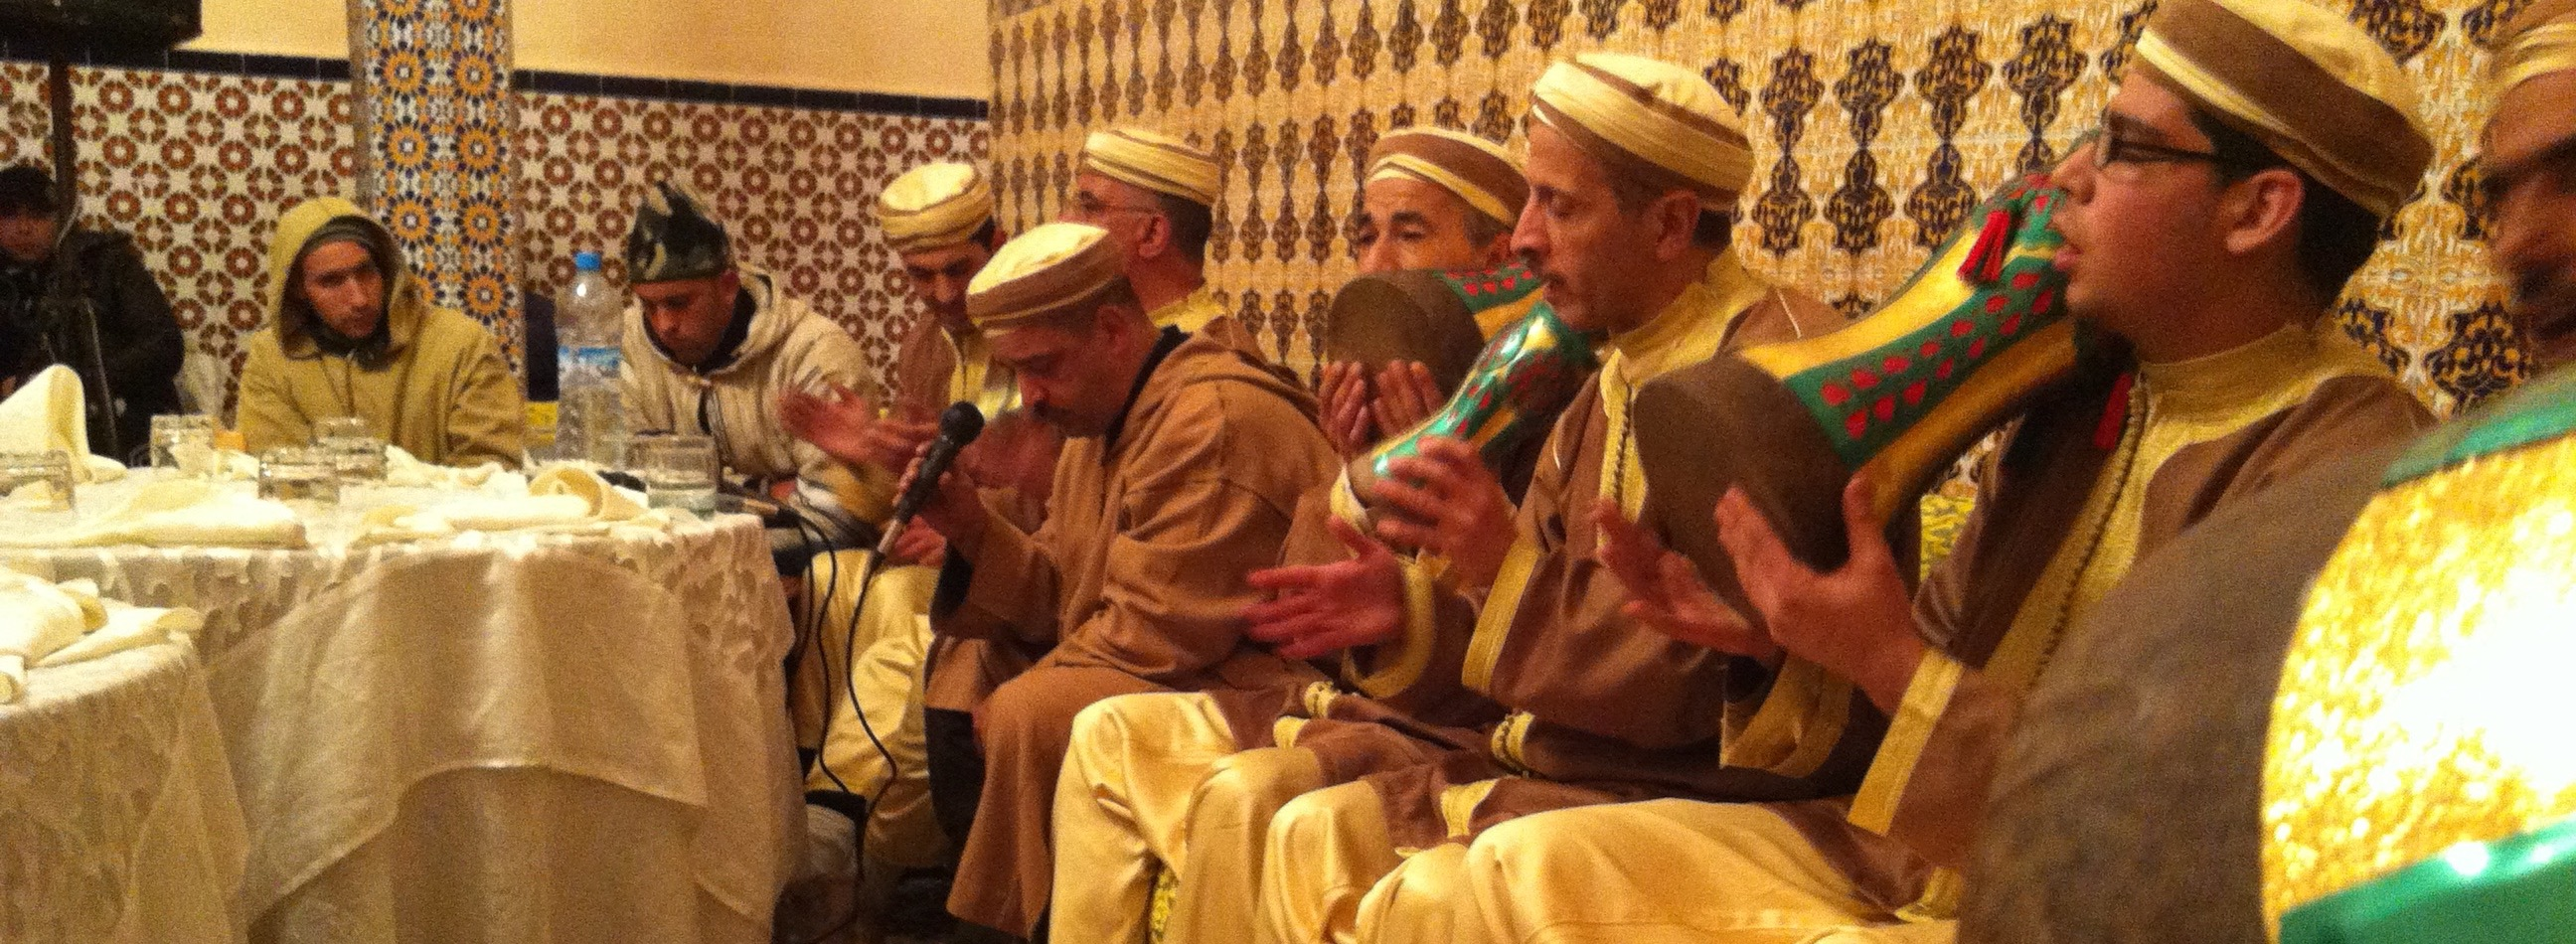
\includegraphics[width=\textwidth]{../../chapters/witulski-rhythm/images/Hamadsha2013.jpg}
  \caption*{Hamadsha ensemble in a performance in 2013}
\end{figure}  

\hypertarget{part-1-expectation-and-repetition}{%
\section*{Part 1: Expectation and
repetition}\label{part-1-expectation-and-repetition}}

So much of music is about expectation. People who make music set these
up by working within and against what a listener is expecting, which is,
in turn, based on shared experience. The result is a series of common
practices or loose guidelines that are commonly called ``rules.'' Much
of music's excitement, confusion, surprise---the richness that makes it
fulfilling in so many ways---derives from how it satisfies or
transgresses our expectations.

\hypertarget{familiarity-unfamiliarity-and-repetition}{%
\subsection*{Familiarity, unfamiliarity, and
repetition}\label{familiarity-unfamiliarity-and-repetition}}

While rhythm is an integral part of all music, it is often foregrounded
in discussions of drumming or percussion. Depending on your musical
experiences and expectations---what you listen to---a drumming pattern
can be confusing, boring, groovy, exciting, and so on. Example 1 is a common
rock beat. Thanks to the globalizing tendencies of the music industry,
this is a familiar sound for many people across the world.

\begin{figure}
  \centering
  
\includegraphics[height=4cm]{witulski-rhythm-part-1.png}
  \caption*{Link for Part 1 (Examples 1-6 and Video Example 1). \wmturlcaption}
\end{figure}

Many different things combine to determine how you might hear and feel
this pattern. Here are some examples:

\textbf{Familiarity:} If you have heard certain types of popular music
before, then this pattern may sound familiar. That does not mean that
you have words to describe it or have ever listened and said ``Oh, I
know that drum pattern, I've heard it before!'' This is an example of
how things like globalization, memory, nostalgia, and culture play out
in listening. If someone remembers her parents listening to a certain
artist or type of music (like
\href{https://www.youtube.com/watch?v=bjCoKslQOEs}{1950s country}, the
band \href{https://www.youtube.com/watch?v=P5jNJd7HRVU}{Blood, Sweat,
and Tears}, or \href{https://www.youtube.com/watch?v=nyYqkRv0D5g}{1980s
hip hop}, for example), then similar little moments in something that is
new to her can bring back old emotions or memories. For country, a
guitar picking technique might trigger a memory. Brass instruments like
the trumpet and trombone in a rock band might take her back to Blood,
Sweat, and Tears. ``Old school'' beat samples may draw out '80s hip hop.
It is nearly impossible to talk about music without these memories and
experiences. The hard part, of course, is that we all live different
lives. Therefore, when we hear something new (or old), we hear it
differently. Even if it's a supposedly ``simple'' rock beat.

\textbf{Unfamiliarity:} If you have no expectations---maybe because
something you hear, see, or taste is brand new to you---it's really hard
to guess what is coming next. But we only have to wait a moment to find
out. With visual art that is static (like a painting), we might take our
time and look more closely at details. We return to what we saw and
think about it differently. Music vanishes into the air as soon as we
hear it. We are left with memories of the sound and of how our bodies
reacted to it. Maybe we danced and felt the movement. Perhaps we are at
a loud live concert where we were pushed around by the sound waves. I
still remember the sensation of how the heavy drums at a
\href{https://www.youtube.com/watch?v=8LhCd1W2V0Q}{Lenny Kravitz}
concert physically shoved my guts to the back of my ribcage when I was
in high school.

\textbf{Repetition:} If the sound repeats, then it is easier to find a
pattern and build an expectation. Of course, it also sets us up as
listeners to be surprised when the repetition ends. And some patterns
show themselves to us more quickly: that, again, is based on what we
have heard before.

In the case of the example above, the pattern is broadly (but not
universally) familiar. It's also repetitive over a short \emph{cycle}, a
single iteration. Cycles can be measured in different ways. A composer
scoring a film might be thinking in terms of seconds or milliseconds to
line up the sound and the video. It is more common, though, to refer to
an internal pulse called a \emph{beat}. That word gets used in many
other ways, though, and we'll leave it for now and come back to it
later.

\hypertarget{organizing-time}{%
\subsection*{Organizing time}\label{organizing-time}}

That earlier pattern is fairly simple (which doesn't mean that it's not
interesting or full of potential creativity). More intricate patterns
with less regular internal relationships can make it harder to grasp
what's happening at first. More significantly, however, is the fact that
there is no single way to hear or feel rhythm, let alone music. Example 2 is
an example from a family of common rhythmic cycles that are common in
African diasporic traditions, especially in Brazil, Cuba, and the United
States. It usually gets played on an instrument that is loud and clear,
since musicians use the pattern to hold everything else together. A bell
of some sort or the \emph{clave}, a pair of sticks, are common
instruments to use. This particular variation is sometimes called the
\emph{rumba clave} after the Cuban rumba (see Moore 2010).

Go back and listen to that again, but try and clap along this time. Just
see if you can work it out. It might be hard, it might be easy. Where
does the cycle start? Can you hear the point where it repeats?

\emph{Really, listen again and try clapping or tapping along. Then try
to stomp or say ``Top'' at the beginning of each cycle.}

Example 3 is an example of this pattern in practice, though it is it hidden
somewhat within the guitar accompaniment. See if you can hear it: \href{https://folkways.si.edu/lydia-mendoza/la-bamba-rumba/latin-world/music/track/smithsonian}{Lydia
Mendoza, ``La Bamba''}.

You might have heard the pattern differently, though. If we move the
starting point to another part of the pattern, it changes the character (Example 4).

Wayne Marshall describes how this pattern is tied to the racialized
history of country music, calling it the ``American clavé'' (Marshall
2020). Flipping it so that the new beginning of the cycle is at the
beginning of the graphic makes it easier to see (Example 5).

Note that the clap to start the pattern happens during a silence. Rhythm
is not just about sound, it's about the creative use of space, too. On
the \href{http://wayneandwax.com/?page_id=9315&fbclid=IwAR02xUOhjtC4fw-E6LOTQzcakI4o2IgKlkHmodg5FAbcr3X7qLmz-wS9FXk}{website accompanying the article}, Marshall shares a long ``megamix''
of songs from across American music history that utilize the same
rhythmic cycle (Video Example 1). Listen for how the pattern organizes time through
repetition and expectation across these songs. It might quickly become
familiar. (It's a long mix, jump around to hear different examples.)

\subsection*{Ambiguous terms}

It's worth discussing the words \emph{rhythm} and \emph{beat} themselves before trying
to use them to talk about other things. People use these words
interchangeably and, in fact, they can mean the same thing. They also
might refer to different, but related, ideas. I separate them here while
recognizing that the language used to talk about these distinctions ``in
real life'' is at least somewhat artificial.

A \emph{rhythm} refers to sounds and silences that are associated based on
their relationship in time. They come together to create a unified
``thing'' that might appear again. Some traditions have well-recognized
names for certain rhythms. When rhythms that are familiar appear in
different contexts, they might gain referential meanings over time.
``Shave and a haircut, two bits'' has become a common ending to songs
during over the last century in America. It was so common that it could
be and satirized. \href{https://www.youtube.com/embed/4W3cPSntmBk}{This short video} has some good examples and discusses
how such a short phrase can build so much anticipation.

The \emph{dembow} rhythm (Example 6) comes from a specific place and has its own history in
the Caribbean (Marshall 2008). Like the examples above, it demonstrates
how repeating a \emph{rhythm} can turn it into a \emph{groove}, to use a
not-so-technical term. This pattern underlines global popular music
styles, especially in genres like \emph{reggaeton}.\footnote{When preparing this, I did a quick search in Spotify for "reggaeton" and found a mix of songs from 2020. Almost every one of them had the dembow rhythm featured prominently in the mix.} \href{https://youtu.be/bZMPz5lzb2U}{``Don Don,'' a 2020 release from Daddy Yankee, Anuel AA, and Kendo Kaponi}, is one of many examples.

One use of the phrase \emph{the beat} refers to the cycles of looping rhythmic
phrases that gives forward momentum to a piece of music. As the next
part describes, the \emph{beat} of a song can also refer to a steady pulse that
we sense in our bodies. The confluence of the pulse and the music that
marks that pulse creates a terminological ambiguity that can be
confusing when writing about sound.

Familiarity, expectation, and ambiguity are more than esoteric musical
ideas. Musicians use them in meaningful ways. Take an example from
electronic music (among other things): the beat drop.

When ``the beat drops'' in a song, the entire groove of the music
dramatically and powerfully changes. That the change happens at a
specific moment (\emph{a beat}) and is caused by changes to the repetition of
rhythms (\emph{the beat}) is not lost on dancers in a club who are anticipating
the drop, ready for the boost of energy. Anticipation, which is related
to expectation, builds as the musician (a DJ in this case) toys with the
sound of the music. The pacing of the music doesn't change, but
something in \emph{the beat} does. It's easier to hear this than to read about
it. It's even better to feel it happen, since rhythm and music are
things that our body reacts to. Let yourself \emph{feel} these sounds as much
as you hear them or see people reacting: \href{https://www.youtube.com/embed/nx8bGoNkvSI}{Skrillex in Argentina}.

\hypertarget{part-2-cycles-of-time}{%
\section*{Part 2: Cycles of time}\label{part-2-cycles-of-time}}

We can divide time into pieces, both small and large. Seconds or minutes
move quickly when compared to hours, days, and weeks. We can count
seconds, but feel hours passing differently. We generally use sleep to
mark days and weather can tell us about passing months or years. The
same is true for music. While writing music down on paper forces us to
measure things in certain ways, those methods are not always aligned
with how we sense sound's temporal momentum.

Most musics around the world, including many European and American
styles, use rhythmic cycles to orient the listener. The rock beat from
earlier shows this: within much popular music, the cyclic repetitions
provide momentum and stability while the subtle variations (like those
in the dance club) manipulate that stability to create anticipation.
This is one reason why popular music can be criticized as ``mechanical''
(see Adorno 1990{[}1941{]}, for an example), but it's also one of the
reasons why it is accessible and engaging.\footnote{Western classical
  music, as it is often taught in schools, focuses on grouping smaller
  divisions of time to create \emph{measures}, also called \emph{bars}.
  The divisions are called \emph{beats}, not to be confused with
  \emph{the beat} (of, say, a pop tune).}

These cycles even have names: a high school jazz band percussionist may
get sheet music with a small label in the upper left hand corner that
says ``samba,'' ``funk,'' ``rock,'' or ``bossa nova.'' These terms refer
to adaptable patterns that the player can learn. They play this cyclic
pattern (``lay down the beat,'' perhaps) and provide a foundation for
the rest of the ensemble. The player is not a machine, though. She will
incorporate nuances and changes to match other things that are happening
across the ensemble or to toy with the energy level of the performance.
The pattern is simply a skeletal guide, a starting place.\footnote{This
  way of thinking about how to organize time in music differs from how
  rhythm and a concept called \emph{meter} are taught in many music
  classrooms. Where the approach I describe here follows the way people
  make, listen to, and feel music in many contexts across the world
  (including in Europe and the United States and in classical music
  traditions), the teaching of rhythm and meter often focuses on
  quasi-mathematical procedures that relate to written musical notation.
  In practice, both in western educational systems and elsewhere, rhythm
  is taught verbally, using syllables. One example that demonstrates how
  an unwritten educational system can represent complex rhythms uses
  syllables like ``takadimi'' to connect and divide rhythms within
  Hindustani music's \emph{tala} system. For more on this particular
  practice, see chapter 4 of George Rucker's \emph{Music in North India}
  (2011). Notation is important for a number of reasons, but there is
  much that it does not represent well, including nuances in rhythm that
  change the ``feel'' of a pattern. Furthermore, centering a specific
  type of notation and transcription can inadvertently reinforce
  problematic ideologies (see Marian-Bălaşa 2005). As seen in the
  maqamworld.com examples that follow, musicians across the world use
  western notational techniques as a tool to represent sound, but they
  recognize its failures and it rarely shows up as a performance tool.
  This, again, is true in ``the west'': innumerable outstanding
  musicians never needed to learn to read music to wield it powerfully.
  Notation is an abstraction that can serve a purpose (namely, it can
  preserve and transmit some elements of sound for distribution,
  analysis, or similar goals). Also relevant is the fact that there are
  many other representational systems available to musicians and
  listeners, not only the one that has roots in European classical
  traditions (see Killick 2020 for one example).}

In many Middle Eastern musical styles, these patterns have similar
names, each with its own history, appropriate place, and connotation.
Johnny Farraj and Sami Abu Shumays describe many of them in \emph{Inside
Arab Music}, but they also outline a selection on their website:
\href{http://www.maqamworld.com/en/iqaa.php}{maqamworld.com}. These
patterns, collectively called \emph{iqa'at}, are made of up two general
types of drum strokes (or other sounds): \emph{dum} signifies a lower,
heavier sound while \emph{tek} is usually higher or lighter.
Maqamworld.com uses the letters \emph{D} and \emph{T} to show these,
with \emph{S} signifying a pause or silence. Take a moment to listen to
the ways in which some of these cycles work in different pieces:
\href{http://www.maqamworld.com/en/iqaa/maqsum.php}{the iqa' called
\emph{maqsum}} is a popular one to start with.
\href{http://www.maqamworld.com/en/iqaa/ayyub.php}{The examples for
\emph{ayyoub}} show a huge diversity of stylistic range within one
pattern. Some, like
\href{http://www.maqamworld.com/en/iqaa/zaffa.php}{\emph{zaffa}} are
specifically linked to certain traditions, in this case a wedding
procession, even though they now appear in other styles and contexts.
Listening to a symphony orchestra presenting popular music, as when
\href{https://www.youtube.com/watch?v=Tb5zO7OybPg}{a group like Black
Violin} incorporates hip hop beats into classical chamber music
contexts, gives an idea of how a rhythmic pattern (a funky hip hop beat)
can hold its identity in a seemingly unrelated context (the classical
music hall).

\hypertarget{layers-of-interaction}{%
\subsection*{Layers of interaction}\label{layers-of-interaction}}

Cyclic rhythmic patterns can grow and adapt in many ways. One is through
improvisation: a musician can subtly change the placement of certain
sounds, add new ones, or remove a few parts of the rhythm to regulate
energy. ``Regulate'' sounds so sterile, it's about getting a crowd hype
or making them hold their collective breath in anticipation. Groups of
people can work together to do the same. If you have ever clapped along
to a piece or changed how you move your feet while dancing, you were
co-creating a pattern. This happens when, at a concert, everyone starts
jumping together or swaying from side to side, cell phone flashlights
held high. Rhythm can draw people in and unite them in a common musical
experience.

Another form of adaptation is layering. A technical term for a repeating
rhythmic pattern is an \emph{ostinato}. When one of these ostinatos
(rhythmic cycles) appears alongside another, they can combine to create
something identifiably new. This is how a drum set works. A pattern on a
bass drum appears alongside a second one on a snare drum, perhaps a
third on a high hat cymbal, and others on floor toms, larger cymbals, or
other instruments to create an intricate groove.

A simple example from my own research in Morocco demonstrates this well
(Witulski 2019). This is a pattern that appears in much popular music,
but I crossed paths with it when researching a sacred ritual tradition
as practiced by the \emph{ʿissawa} brotherhood.\footnote{In this case,
  the term ``brotherhood'' refers to the all male musical ensembles who
  carry out ritual ceremonies. The events themselves are usually open to
  client families (who require healing through sacred blessing) and
  their friends.} It is part of a religious healing ceremony that
involves prayer, possession trance, devotional singing, and plenty of
dancing for fun. This rhythm animates the moments where the musical
ensemble invites laughter and popular religious songs into the long
night's event. It also appears in a tradition of sung poetry called
\emph{malhun} that includes both ``sacred'' texts and ``secular'' ones
(Magidow 2016).

In \emph{ʿissawa} contexts, musicians articulate this pattern on a pair
of clay drums that are tied together. Some artists have switched from
these traditional drums, however, to use manufactured \emph{timbales}.
In both cases, a larger and smaller drum makes two distinct sounds: one
is lower and the other is higher. In \emph{malhun}, different musicians
each have small handheld goblet-shaped drums. Each one, called a
\emph{tarʿija} has a slightly different sound because of the natural
fish-skin head. This video shows another brotherhood, the
\emph{hamadsha}, who borrow from both of these styles within their own
ceremony. I recorded this in Meknes in 2013. The group is led by
Abderrahim Amrani and features a guest, Mohammad Essousi, who is a
prominent \emph{malhun} singer (Video Example 2).

In Example 7, drums and clapping articulate two main rhythmic
patterns. The first is two notes, equally spaced. The second is offset
and the notes are unequally spaced. They are layered to build a new
pattern, one that is coincidentally similar to reggaeton's
\emph{dembow}.

\begin{figure}
  \centering
  
\includegraphics[height=4cm]{witulski-rhythm-part-2.png}
  \caption*{Link for Part 2 (Examples 7-8 and Video Example 2). \wmturlcaption}
\end{figure}

Combining the two patterns changes the overall rhythmic cycle's feel.
They integrate into a single idea, yet people still clap along to one
pattern or the other, as in the video. Try identifying and clapping the
distinct patterns when listening to the two of them together, then mute
each (in Example 8) and try to clap the other. It may be easier to go back to the video
and clap along with the musicians.

These are mechanical examples produced by a computer. The real
participants in the video changed the patterns in other ways, as well.
For one, it is common to speed up when approaching the climactic ending
of a section of poetry. As they accelerate, musicians subtly adjust the
relationships between the two patterns. They might make the last note of
the second pattern louder to push listeners back to the beginning of the
cycle. When I am at a ceremony or concert, I can feel this rushed
anticipation in my body. They might squeeze the two middle notes, which
are already close together, even tighter to excite the music further. We
turn toward these details next.

\hypertarget{part-3-feeling-the-beats}{%
\section*{Part 3: Feeling the
beat(s)}\label{part-3-feeling-the-beats}}

Just as musical repetitions and relationships can orient listeners over
long stretches of time, smaller details impact how we feel music in the
moment. Some of these details go unnoticed in common discussions of
sound. For example, they may not appear in written music notation in
western contexts. That doesn't mean that they are not important or that
we don't feel them.

Much of the world's music has a sense of \emph{pulse}, a consistent
sense of motion. This is one of many terms that is difficult to describe
in words without falling back on other equally problematic sets of
terminology. It also resists being bounded into a specific definition.
Take dance: a pulse can be the points in time where you put your feet
down or, in the case of Argentinean tango music, where you step while
walking. \href{https://www.youtube.com/embed/wIvfPI_GT3U}{Listen here
and watch} as the dancers' feet move in a somewhat consistent pulse, or,
to use another term, to a beat.

That word, \emph{beat}, returns here. The \emph{pulse} is often referred
to as the \emph{beat}, but I will nudge the meaning here to say that
each pulse---each moment in time---is a \emph{beat}. These beats that
make up the pulse are not identical to the rhythm, though in Western
music notation systems, they do get used to calculate larger structures
like \emph{meter}.

One striking aspect of the \emph{pulse} and \emph{beats} in a piece of
music is that listeners can sense them, even if no sound happens at
those moments in time. They are not explicitly aligned with strikes on a
drum or chords on a guitar. They exist among and between sounds. They
are perceived, imagined, and based on our expectations.

Listen to this rhythm (Example 9). The consistent pulse is explicitly presented
between the two instruments (a bass drum and snare drum). Try clapping
the consistent \emph{pulse} that is marked in blue boxes along with the
rhythm.

\begin{figure}
  \centering
  
\includegraphics[height=4cm]{witulski-rhythm-part-3.png}
  \caption*{Link for Part 3 (Examples 9-17 and Video Examples 3-5). \wmturlcaption}
\end{figure}

In this case, every beat of the pulse (at least as I hear it) is played
by one of the instruments. Here's another example that's similar. Try
clapping along again. In this case, you can see the consistent pulse
highlighted in blue outlines, but you can also \emph{feel} it, even when
the bass drum does not specifically articulate it (Example 10). (Listen without the
pulse, then you can use the button to add it in.)

This time, the beat in the middle of the repeating pattern is not
articulated, but you may have still felt it and clapped during the
space. Your body moves the same way and the clap feels appropriate
there. This is the result of \emph{syncopation}, an emphasized sound
that does not appear on a regular beat or at an expected moment. In this
case, the bass drum hit shows up before the expected beat.

As stated above, this is not just about drums. Here are some lines that
could be in a funk band horn section (Example 11). Even without the rest of a group,
you may be able to feel the beat. They both have some syncopation, but
the second one has even more. Yet, the pulse is still there (even if
it's harder to feel out of context).

Not all music has an underlying pulse. When a musician performs
``freely'' and without adherence to a consistent pulse, it can be termed
\emph{free rhythm}. This happens in solo introductions to a piece of
music that showcases a performer's virtuosic and expressive technique.
Without an underlying consistent pulse, a musical idea can still toy
with related ideas like \emph{pacing} to generate motion and tension. By
moving from slow to fast or suddenly shifting the momentum, free rhythm
can generate a powerful feeling of rhythmic direction.

\hypertarget{grouping-beats}{%
\subsection*{Grouping beats}\label{grouping-beats}}

Even when the pulse is fairly consistent, we don't hear music as a
steady stream of even sounds. It's possible to intentionally give that
sensation of mechanical consistency to listeners, but usually we hear
and feel weight in different places as we find patterns by grouping
beats together. These groupings comprise the concept of \emph{meter},
though that term can be tied into music notation in ways that are not
always helpful. Like so much else here, these are easier to hear or feel
than they are to describe.

Most groupings are either sets that are multiples of two (\emph{duple})
or three (\emph{triple}). They can be combined to make innumerable other
possibilities. They can also both happen at once. Most popular music is
duple: rhythmic patterns like the ones described above overlay a pulse
of evenly grouped beats. That does not mean that we all hear the same
duple groupings: I might hear groups of 4 quick beats where you hear 2
slow ones. Unless you are trying to write music down, that distinction
is unimportant. Here is a loop with a clave sound that divides the pulse
in two different ways, but they are both duple (Example 12).

Each group is called a \emph{measure} or \emph{bar} and where those
measures start and end can be arbitrary. In the above example, someone
could feal each iteration as one bar or made up of two shorter ones.

Triple groupings \emph{feel} different. Here is an example from the
American old time fiddling tradition as performed by Tommy Jarrell, an
influential fiddle player (Video Example 3). Try counting ``one, two, three, one, two,
three\ldots{}'' as he plays. A lifting or lilting sensation is at the
core of many triple meter pieces, in part because of the dance steps
that the music accompanies.

If the pace quickens, though, we might feel the central pulse somewhere
else. In this short sample of an Irish jig, a patting sound marks the
beat. Counting ``one, two, three'' quickly still fits well, but a dancer
cannot move her feet at that speed. Instead, you step to a slower ``one,
two.''

\href{https://folkways.si.edu/wendy-macisaac-fiddle-jackie-dunn-macisaac-piano/the-short-grassjig/the-braes-of-elchies-jig/traditional-jig/gallaghers-jig/the-pibroch-of-odonal-dubh/celtic-old-time-world/music/track/smithsonian}{``The
Short Grass Jig'' by Wendy MacIsaac, Jackie Dunn MacIsaac}

We can also add sets of duple or triple groupings to make more
complicated ones. Arabic music has a classical form called \emph{samaʿi}
that is technically ten beats. In practice, however, it is a group of
three beats followed by a group of four (or two pairs), and then another
group of three (Example 13).

These groupings can appear in ways that foster ambiguity and generate
tension for the listener. Rhythms can spread over time in a way that
emphasizes two or more different pulses simultaneously. This
displacement can be troubling or exciting. Stephen Friedson argues that
it opens the body to an experience of trance (1996). Ann Danielsen
describes how the guitar groove in James Brown's famous song ``Sex
Machine'' creates its own pulse that is slightly offset from the main
one followed by the rest of the band (2006). While it does not bring
about trance, it gives life to funk. In either case, a similar musical
practice impacts the listener in a contextually-defined way, but both
change our perception (Becker 2004).

Listen to Example 14 and clap along to the pulse that you hear. Then
try clapping to a different one by clicking the button. If you are up to
the challenge, try shifting your perception from one to the other and
back. At first, it might feel unnatural. Eventually, and with
familiarity, it may get easier.

\hypertarget{dividing-time}{%
\subsection*{Dividing time}\label{dividing-time}}

Just as beats are organized into larger groups (measures), they are
divided into smaller parts. Of all of the rhythmic concepts discussed
here, this might be the one where notational practices in western
tradition struggles the most to depict the sounds that we hear. Sounds
that land between beats rarely come at mathematically consistent
intervals. Instead, a musician's expressivity will push a note just
before or after, making it subtly early or late.

The consistent division of beats that creates an expectation for
listeners is called the \emph{subdivision}. The nudges that happen in
practice usually go unspoken, but some analysts and music theorists call
it \emph{microtiming}. Subdivisions are somewhat straightforward to talk
about. Microtiming involves a level of nuance that can be far more
difficult to articulate.

In western music theory practice, subdivision is generally taught as
\emph{duple} or \emph{triple}, just like meter and measures (the larger
grouping of beats). A duple subdivision divides each beat into two even
halves or some other multiple of two (like four quarters). A triple
subdivision divides them into three. Like the pulse itself, these
divisions are not always made explicit in the music: they are structures
we perceive as listeners.

The following examples present these structures as connected levels of
organization. When listening, you can use the buttons to have the loop
articulate different ``scopes'' (the measure/grouping of beats, the
pulse/beats, and the subdivision/division of beats).

Note that since these are real audio examples, they don't line up
perfectly. The performers subtly shift their timing, even over a short
period. Example 15, which demonstrates a duple feel, is a version
of ``St.~Louis Blues'' by Jim Reese Europe's ``Hellfire Band.'' Europe
was a popular and successful black bandleader in the early 20th century
who led a military band during World War I.

Example 16, with beats grouped into sets of three and divided
into duple subdivisions, is from American fiddle music.

\hypertarget{playing-with-subdivisions}{%
\subsection*{Playing with
subdivisions}\label{playing-with-subdivisions}}

In practice, musicians manipulate these divisions further. \emph{Swing}
is one common example that developed as part of the early jazz scene in
the United States before the word came to represent its own genre of
music. In swing, a duple subdivision turns into something else: the
musicians lengthen the first half and shorten the second half. This
means that they are no longer halves.

Musicians make use of the flexibility that live performance
offers.\footnote{It should be said that flexibility in subdivisions and
  other expressive techniques are not exclusive to human performers.
  Electronic music has this capability and, in some cases, can do so
  with more specific intentionality on the part of the composer or
  producer.} Swing performers themselves vary the degree of their swing
to create an individual style. Even within a single musical line, they
change the ratios of their subdivisions to build and release tension
(Benadon 2006). Christine Gerischer shares similar ideas about Brazilian
samba music, showing that this is not unique to the genre known as
``swing'' (2006). These manipulations are examples of
\emph{microtiming}, adjusting the timing of notes in slight, but
noticeable, ways.

These adjustments can sound and feel different. As a basic
demonstration, move the slider to change the subdivision ratio and
listen to how the simple swing drum set beat responds (Example 17). Then, see if you
can hear or feel the swing in Count Basie's ``One O'Clock Jump'' (Video Example 4). (It's
not always easy to hear, but you may feel like there's some forward
momentum that you can't quite articulate. That's fine! In fact, that's
the point!)

A frequent division of the beat that is related to swing involves a
first ``half'' that is roughly two-thirds of the length of the beat,
leaving one-third for the second ``half.'' This particular division
turns into a mathematical \emph{triple} subdivision where the first two
thirds are linked together and roughly aligns with another name: a
\emph{shuffle}.

This example from Odetta, a folk singer and Civil Rights activist in the
1950s and 1960s, is a slow shuffle, which brings it closer to the sound
of the blues (Video Example 5).

This technique of rushing or delaying notes can happen anywhere in a
piece of music, but it is a matter of balance. Breaking too far from
expectations or norms could confuse a listener or dancer, but sticking
to them methodically might get dull. One of my own favorite moments that
exemplifies this is from
\href{https://www.youtube.com/embed/zJuX-JJ8WF0}{a performance of
``Watermelon Man'' by Mongo Santamaria}. While listening, try to let
yourself feel the groove and, if the music inspires you, move along with
it or clap. Then, \emph{feel} how the percussion (drum set and other
instruments) almost pull the horn section (the brass instruments and
saxophone) along. It is even more extreme when the percussion drops out
at about 30 seconds in. When I listen, I can't help but to actually feel
this tension in my body, as well as the relief that comes when they snap
back together.

The final section turns to Morocco for a series of rhythms that
challenge expectations by combining each of these practices.

\hypertarget{part-4-consistent-inconsistencies-from-morocco}{%
\section*{Part 4: Consistent inconsistencies from
Morocco}\label{part-4-consistent-inconsistencies-from-morocco}}

As mentioned in the opening of this series, one of my main goals here is
to disassociate widely used terminology from an exclusive understanding
based in western classical music and its associated system of written
symbols.\footnote{The symbols that I refer to here include ``standard''
  notation. These systems and the organizational logics that underpin
  them can influence many musical activities, including
  pedagogy/teaching and analysis/transcription. Transcription is the act
  of notating sounds and, while it often refers to writing out spoken
  words (transcribing language), it can also involve using some
  notational system to transfer music into a static and written form. It
  can be a powerful tool for preserving music, as demonstrated by
  composers ``notating'' their musical ideas for the convenience of
  performers, and musical analysis.} Rhythm is central to music
worldwide, even in contexts where it is important in absentia like free
rhythm improvisations. It is difficult to imagine music that does not
incorporate a sense of passing time. Even where that might be possible,
it is likely to work by breaking expectations.

The exclusive association of ideas like beat and meter to western
systems has a secondary impact: it leads analysts to consider all music
from a perspective that adheres to western traditions. Using three
examples from my own research in Morocco, I aim to demonstrate how
centering experience and perception and decentering prescriptive
conceptions of musical elements brings about new ideas of how music
works.\footnote{While my research was ethnographic fieldwork over
  roughly three years in Morocco, these observations are my own. I hope
  to take the ideas I present here back to Morocco and make them central
  to interviews and conversations to see whether they are shared by
  Moroccans who live these musical traditions. This is methodologically
  difficult in part because the terminologies used by musicians trained
  in western systems (wherever they might live and work) do not always
  align with how listeners talk about music.}

\hypertarget{uneven-beats}{%
\subsection*{Uneven beats}\label{uneven-beats}}

Two of these three examples come from the \emph{hamadsha} tradition. The
hamadsha brotherhood is a Muslim Sufi group, which means that they
regularly gather to perform and participate in sung devotional poetry.
Unlike some other Sufi brotherhoods, the hamadsha are organized as
professional ensembles who visit client houses to chant and sing poetry
along with instrumental accompaniment. They are closely linked to the
figure of Aisha, a spirit who possesses some individuals. The ritual
healing ceremony is not an exorcism. One of its goals is the maintenance
of the relationship between Aisha and her host body. The musicians and
their ceremony help the client to appease Aisha through chanting,
prayer, singing, a trance possession ``dance,'' and the ritual sacrifice
of animals like chickens and goats.\footnote{For more detail on the
  hamadsha and their ritual ceremony, see Witulski 2019.}

An evening hamadsha event moves through a number of segments, each with
its own musical characteristics. One, called the \emph{saf al-ginbri}
features an underlying rhythmic pattern of uneven heavy beats. This
pattern is also common elsewhere in the world, including the Balkan
region of Europe and across the Middle East (Goldberg 2020). This
example is from a ceremony I attended with the hamadsha leader
Abdderrahim Amrani (Audio Example 1).

\begin{figure}
  \centering
  
\includegraphics[height=4cm]{witulski-rhythm-part-4.png}
  \caption*{Link for Part 4 (Examples 18-22 and Audio Examples 1-3). \wmturlcaption}
\end{figure}

A western system would define this as a 5/8 meter by focusing on the
consistent pulse. In practice, however, this is felt at the larger
grouping of one short beat (subdivided in half) and one that is slightly
longer (made up of three subdivisions). Is it a consistently uneven
pulse (which would be consistent in its own way) or is this an example
of two smaller groupings combining (Example 18)?

I argue that there is no ``correct'' way to hear this. The western
notational practice of calling something like this 5/8 (five even beats
grouped into two and three), however, obfuscates what we hear by
prioritizing written convenience. It fits better into a system built for
western classical tradition that way.

\hypertarget{shrinking-beats}{%
\subsection*{Shrinking beats}\label{shrinking-beats}}

A second pattern is both more complicated from the perspective of
western musical systems and far simpler when understood on its own
terms. It comes from another Moroccan ritual healing ceremony that is
part of the \emph{gnawa} tradition. This music is widely associated with
Morocco's history of slavery and the sub-Saharan Africans who were
forcibly brought to the country across the Sahara from West Africa. This
ritual also serves to heal clients by repairing the relationship between
them and possessing spirits, but here Aisha is just one of many. As with
the hamadsha, the ceremony moves through various segments. These are
associated with specific colors (black, white, blue, and so on) that
identify individual spirits or sets of spirits who might possess the
client. The music of each segment is specific to that spirit, but it is
more broadly similar throughout the evening than the more varied music
that animates the hamadsha ceremony.

Gnawa music uses three types of instruments. A single low bass string
instrument called a \emph{hajhuj}, \emph{ginbri}, or \emph{sintir} is at
its core. This is the only melodic instrument that accompanies singing.
A large drum called a \emph{tbal} appears in certain places. Of interest
here, though, are the \emph{quraqib}, sets of iron castanets that beat
out consistent rhythmic patterns throughout most of the overnight
ceremony.

\begin{figure}
\centering
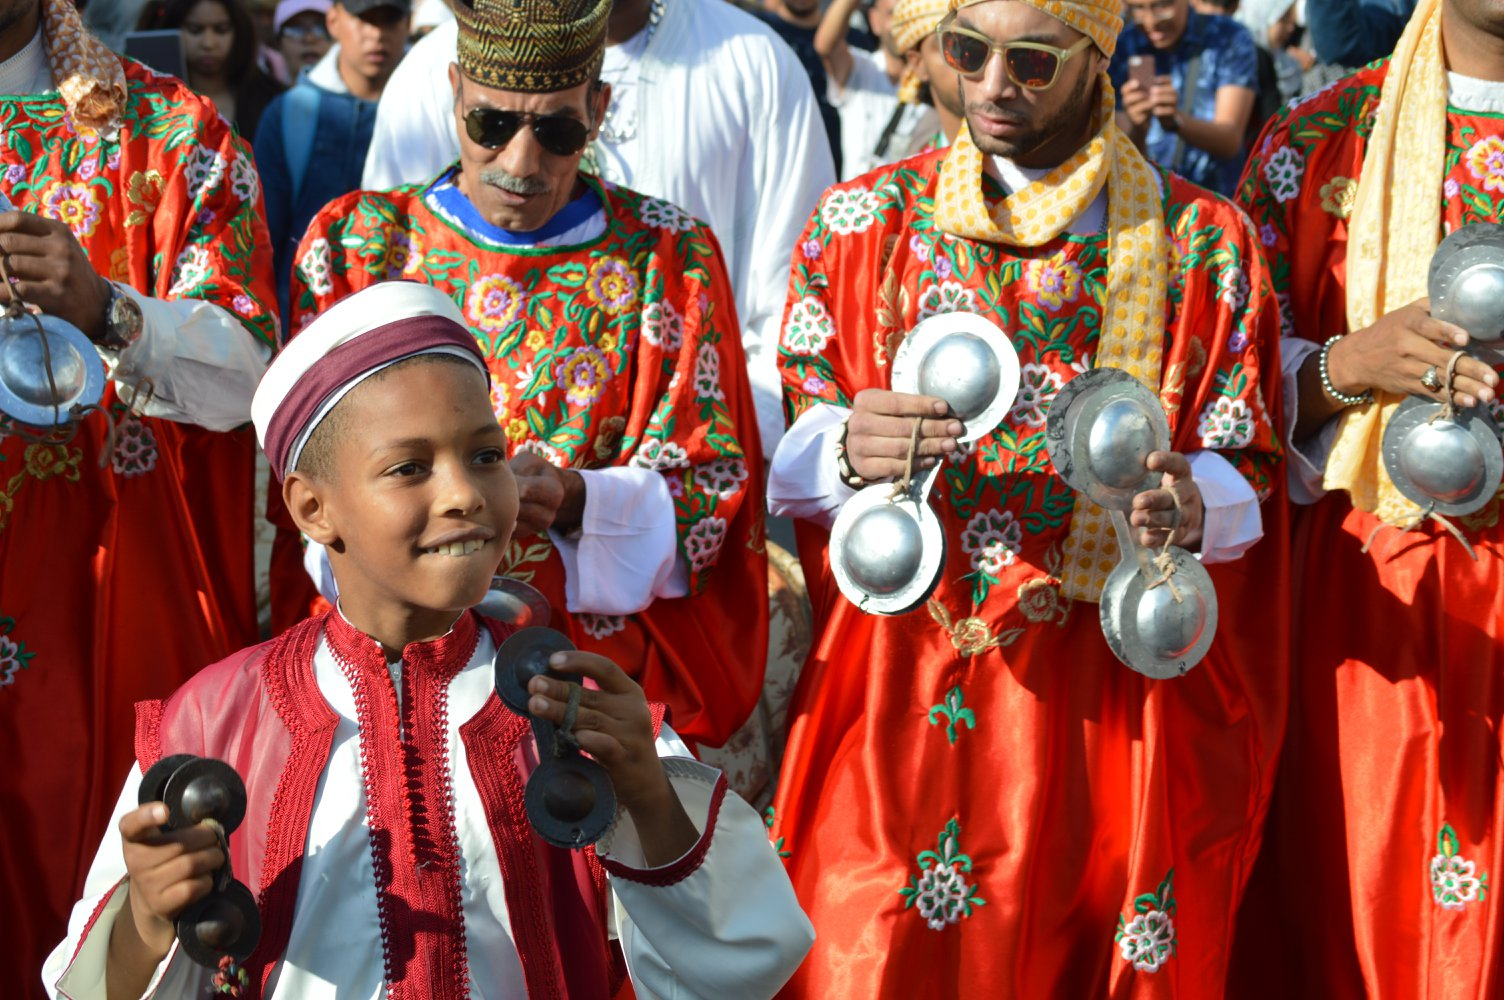
\includegraphics[width=\textwidth]{../../chapters/witulski-rhythm/images/gnawa.jpg}
\caption{Quraqib, as demonstrated by members of Mʿallem Said Oughessal's
gnawa troupe during the opening parade of the 2018 Essaouira gnawa and
world music festival}
\end{figure}

Most individual songs in gnawa music start slowly and get faster as the
trance intensifies.\footnote{If using western terminology, the speed
  would be referred to with the term \emph{tempo}.} This example---and
many similar instances of speeding up gradually that happen across the
globe---is different than most western instances where, for example,
acceleration may happen at the end of a piece to build excitement. When
it does happen in western traditions, the internal subdivision pacing
increases with the speed of the beats. This maintains the relationships
between them (at least roughly). A duple subdivision usually stays
duple.

At higher speeds, it can get hard to maintain the pace of subdivisions
simply because shorter notes get too fast to play. This pacing issue is
simply accepted and normalized in gnawa music. The pattern that starts a
piece gets so fast that the musicians ``even out'' the distance between
the subdivisions. Mathematical ratios are less important than the
intensity of the experience. A gradual moves happens where a feeling of
a duple subdivision shifts into a triple one as longer notes shorten.
This example, whch was played by Abderrahim Abderrazak, my teacher
during my fieldwork in Fez, Morocco, shows the progression. Skip around
the entire track and listen for the difference between the rhythmic
pacing of the beginning and the end (Audio Example 2).

Example 19 lets you change the pacing yourself. You can see how it
goes from feeling like an even duple subdivision to a triple one as you
shorten the first note in the pattern. That also quickens the looping
repetitions.

Western notation easily represents the duple subdivision of the
beginning and triple of the ending, but the gradual change throughout
the song means that most of what brings a person into trance cannot be
so easily written down. The subdivision relationships here are not a
result of a larger conceptual framework. They come from a group of
people who are playing as fast and intensely as they can so that their
music will invite a spirit into the room and heal a listener. In this
way, what we hear reflects a specific set of priorities.

\hypertarget{poetic-license}{%
\subsection*{Poetic license}\label{poetic-license}}

The final rhythm I present here animates two different segments of the
hamadsha brotherhood's ritual (Example 20). \emph{Al-unasa al-saghira} comes first
and features this pattern articulated with clapping. \emph{Al-unsasa
al-kabira} returns later in the evening and uses drums. Both segments
focus on sung devotional poetry that aligns with a rhythmic pattern of
five beats (or five claps) that can be loosely described as short, long,
short, short, long.

One of the core assumptions about rhythm in western-centric systems of
understanding is that the pulse is made up of evenly-spaced
beats.\footnote{There are some common exceptions, including when the
  tempo changes. The tempo is the rate of passing beats or the speed of
  the underlying pulse. When it increases, beats will ``speed up'' and
  the time between them gets shorter.} In fact, this pattern can be
mathematically broken down and written in western notation. The ``long''
beats are equal to three halves of the short beats, as demonstrated by
this example's added imaginary pulse (Example 21).\footnote{Alternatively, these
  embedded examples can be understood as alternative forms of notation.
  While the long and short bars that represent the notes ignore much of
  what western notation includes, they show duration more intuitively
  (in some ways). Notation itself is an effort to foreground certain
  elements of sound that are deemed important by composers, researchers,
  listeners, performers, and so on. Alternative notation is common in
  all forms of music, including western classical music, where the work
  of John Cage, George Crumb, and Krzysztof Penderecki include commonly
  taught examples. Creating your own form of graphic representation of
  sound (notation) is a useful exercise for understanding how these
  decisions and priorities play out in practice.}

Imagining this pattern as comprised of twelve beats makes it easy to
create groupings of two and three. This aligns with the first hamadsha
rhythm that I introduced earlier. It fits into western notation (using
quarter notes and dotted quarter notes), but I argue that it fails to
account for the clearly-defined nature of how these rhythms are
articulated and perceived.

An example of a common variant that ornaments this pattern shows that
this even pulse does not represent how the rhythm works in practice.
Abderrahim Amrani and Fredrick Calmus, members of the brotherhood I
worked with most closely, taught me this drum pattern that organizes and
underlies the entire poetic segment of the ritual (Example 22).

There are two characteristics of this poetic accompaniment that are
noteworthy here. First, the beat or pulse is consistent in that it
repeats over and over again, but not every beat within it is the same
duration. Second, the subdivision stays duple (beats are divided in two)
whether the beat is short or long. This makes some subdivisions longer
and some shorter.

Perhaps this is an example of \emph{syncopation}, discussed earlier. If
we understand the subdivision to be consistent and even (as done in the
above example), then the drum strokes that divide the long spaces are
syncopated. They are between beats.

This pattern repeats over and over throughout the long poetic
recitation, however. While it may feel syncopated at first, the listener
grows accustomed to its asymmetry. If we allow for a pulse of uneven
beats (some long and some short) with subdivisions that divide them in
half instead of mathematically attempting to fit this into a structural
conceptualization designed for a different set of musical traditions,
then we can more closely approximate what is happening. This may sound
syncopated to you. Or you might hear it as regular and expected, despite
its unevenness. The point is not that one is correct: we all hear and
feel music differently. Instead, the point is that we do not need to
prioritize western-centric tools that might not fit the job. Try
listening to the last example again and let it loop for a while. See if
it starts to ``sink in'' over time and feel different.

Up until now, I have been using electronically created beats to
demonstrate this pattern. In practice, however, there is an additional
nuance. The last beat of the cycle is late. This is an example of
microtiming, similar to Mongo Santamaria's ``Watermelon Man.'' This
subtle play with time that can build and release tension happens in
every iteration of the pattern. It becomes a core part, though the
amount of delay is open for exciting interpretation (Audio Example 3).

\hypertarget{conclusions}{%
\section*{Conclusions}\label{conclusions}}

This set of short essays considers rhythm from the perspective of
expectation and ambiguity. Music is something that we feel as much as we
hear. It impacts us, in part, through how we sense it, not just how we
hear or think about it. Rhythm works, in part, by organizing time. This
final section demonstrates how we experience and understand rhythmic
ambiguity and how common ``rules'' and western classical music-oriented
understanding of rhythm can be reductive, failing to illuminate how we
\emph{feel} music.

Music and musicians set up and break down listener expectation in
innovative ways and these dramatically change how we experience music.
Like so many other things, music lives in systems that we internalize,
but, as I hope is clear through these essays, it is at its best when we
understand that the rules of those systems are made to be broken.

\hypertarget{references}{%
\section*{References}\label{references}}

\begin{hangparas}{15pt}{1}

Adorno, Theodor. 1990. ``On Popular Music.'' In \emph{On Record: Rock,
Pop, and the Written Word}, edited by S. Frith and A. Goodwin. New York:
Pantheon Books.

Becker, Judith. 2004. \emph{Deep Listeners: Music, Emotion, and
Trancing}. Bloomington: Indiana University Press.

Benadon, Fernando. 2006. ``Slicing the Beat: Jazz Eighth-Notes as
Expressive Microrhythm.'' \emph{Ethnomusicology} 50 (1): 73--98.

Danielsen, Anne. 2006. \emph{Presence and Pleasure: The Funk Grooves of
James Brown and Parliament}. Middletown, CT: Wesleyan University Press.

Farraj, Johnny, and Sami Abu Shumays. 2019. \emph{Inside Arabic Music:
Arabic Maqam Performance and Theory in the 20th Century Middle East}.
New York, NY: Oxford University Press.

Friedson, Steven M. 1996. \emph{Dancing Prophets: Musical Experience in
Tumbuka Healing}. Chicago: University of Chicago Press.

Gerischer, Christiane. 2006. ``O Suingue Baiano: Rhythmic Feeling and
Microrhythmic Phenomena in Brazilian Percussion.''
\emph{Ethnomusicology} 50 (1): 99--119.

Goldberg, Daniel. 2020. ``What's the Meter of Elenino Horo?: Rhythm and
Timing in Drumming for a Bulgarian Folk Dance.'' \emph{AAWM Journal} 7
(2): 69--107.

Killick, Andrew. 2020. ``Why Global Notation?'' \emph{Global Notation:
Visualizing the World's Music}. 2020.
http://globalnotation.org.uk/why-global-notation/.

Magidow, Melanie. 2016. ``Trending Classic: The Cultural Register of
Moroccan Malhun Poetry.'' \emph{The Journal of North African Studies} 21
(2): 310--34.

Marian-Bălaşa, Marin. 2005. ``Who Actually Needs Transcription? Notes on
the Modern Rise of a Method and the Postmodern Fall of an Ideology.''
\emph{The World of Music} 47 (2): 5--29.

Marshall, Wayne. 2008. ``Dem Bow, Dembow, Dembo: Translation and
Transnation in Reggaeton.'' \emph{Lied Und Populäre Kultur / Song and
Popular Culture} 53: 131--51.

---------. 2020b. ``Ragtime Country: Rhythmically Recovering Country's
Black Heritage.'' \emph{Journal of Popular Music Studies} 32 (2):
50--62.

Moore, Robin. 2010. \emph{Music in the Hispanic Caribbean}. Experiencing
Music, Expressing Culture. New York and Oxford: Oxford University Press.

Ruckert, George. 2011. \emph{Music in North India: Experiencing Music,
Expressing Culture}. Global Music Series. New York, Oxford: Oxford
University Press.

Witulski, Christopher. 2018. \emph{The Gnawa Lions: Authenticity and
Opportunity in Moroccan Ritual Music}. Public Cultures of the Middle
East and North Africa. Bloomington, IN: Indiana University Press.

---------. 2019. \emph{Focus: Music and Religion of Morocco}. New York
and London: Routledge.

\end{hangparas}

\end{document}